\speciestitle{Geopotential Height}{GPH}{GPH}{%
\item[Useful range:] 261\,--\,0.001\,hPa
\item[Contact:] Michael J. Schwartz,
  \email{Michael.J.Schwartz@jpl.nasa.gov}}
\label{sec:StandardGPH}%

\subsection*{Introduction}

Geopotential height (GPH) is retrieved, along with temperature and the
related assignment of tangent pressures to limb views, primarily from
bands near O\cs2 spectral lines at 118-GHz and 234\,GHz.  \thisv GPH
product is taken from the CorePlusR3 retrieval phase that also produces
a number of standard products dependent upon radiances of the 240-GHz
radiometer while the previously released v02.2x and v03.x GPH products
were taken from a preliminary ``core'' retrieval phase.  Despite this
difference, the \thisv GPH product is quite similar to the v03.x product
and to the v02.2 product described in \citet{SchwartzEtal08}.

The heights of surfaces of constant geopotential is a property of the
Earth's magnetic field and does not depend upon atmospheric conditions.
Differences in geopotential between surfaces between surfaces are equal
to the integral with height of the gravitational acceleration, $g$.  GPH
is integral of $g$ with height from the Earth surface geopotential to a
given surface, scaled by $g_0$, the standard gravitational acceleration
at mean sea level, to give units of height.

MLS retrieves on pressure surfaces, and the pressures of GPH surfaces do
depend upon temperature and height through hydrostatic balance and the
gas law.

\begin{equation}
\frac{1}{g_o} \int g\,dh = \frac{R}{M g_o}\int T\,dP/P,
\end{equation}

where $M$ is the molar mass of air and $R$ is the gas constant.

MLS retrievals use the 100-hPa surface as a reference level from which
integrations are performed because MLS does not retrieve temperature
down to the Earth's surface.  Differences of GPH from the 100\,hPa
reference surface used by MLS are equal to the integrated temperature
with respect to log-pressure between the levels, scaled by $R/M/g_0$,
where $R$ is the gas constant, $M$ is the molar mass of air, and $g_0$
is mean sea-level gravity.  Only one element of GPH (chosen to be the
value at 100\,hPa in the MLS Level~2 processing) is independent of the
temperature profile.  Table~\ref{tab:GPHSummary} summarizes the
measurement precision, modeled accuracy and observed biases.  The
following sections provide details.

\subsection*{Biases}
Comparison of MLS retrieved 100-hPa with that of GEOS-5 reveals
persistent and seasonally-varying biases that can exceed 300\,m, much
larger than systematic uncertainties in GEOS-5 100-hPa GPH.  Results
shown in this section are between GEOS-5.2 and MLS v03.3x GPH, but are
beleived to be generally consistent with those of \thisv GPH.

MLS calculations are made assuming that the the World Geodetic System
1984 ellipsoid (WGS84) as the Earth's surface, whereas GEOS-5 uses a
reference geoid,the Earth Gravitational Model 1996 (EGM96), a model of a
geopotential surface.  The use by MLS of the simplified model, WGS84, in
its ray-tracing calculations is reasonable in that retrievals are made
on pressure rather than height surfaces and in that atmospheric opacity
at the frequencies at which MLS observes are such that MLS does not
``see'' the Earth's surface, so accurate representation of its height is
not important for tracing of reflected rays.  However, MLS \thisv and
previous versions of GPH are reported as heights \emph{from the WGS84}.
Comparisons of the WGS84 with a reference geoid
(Figure~\ref{fig:geoidheight}), show differences that can exceed 100\,m.
Ideally, these biases should be subtracted from MLS GPH on pressure
surfaces before (for example) geostrophic winds are calculated from GPH
gradients.
\begin{figure}
\centering\includegraphics[width=0.7\linewidth]{figures/geoidheight}
\caption{The height of the EGM96 geoid from the WGS84 ellipsoid.  These
  values should be subtracted from MLS GPH reported values to give
  geopotential heights referenced to the Earth's mean sealevel
  geopotential. (I will remake this figure as a native eps.)}
\label{fig:geoidheight}
\end{figure}

After removal of the geoid correction, there remain latitudinally and
seasonally-varying biases between MLS and GEOS-5   
\begin{figure}
\centering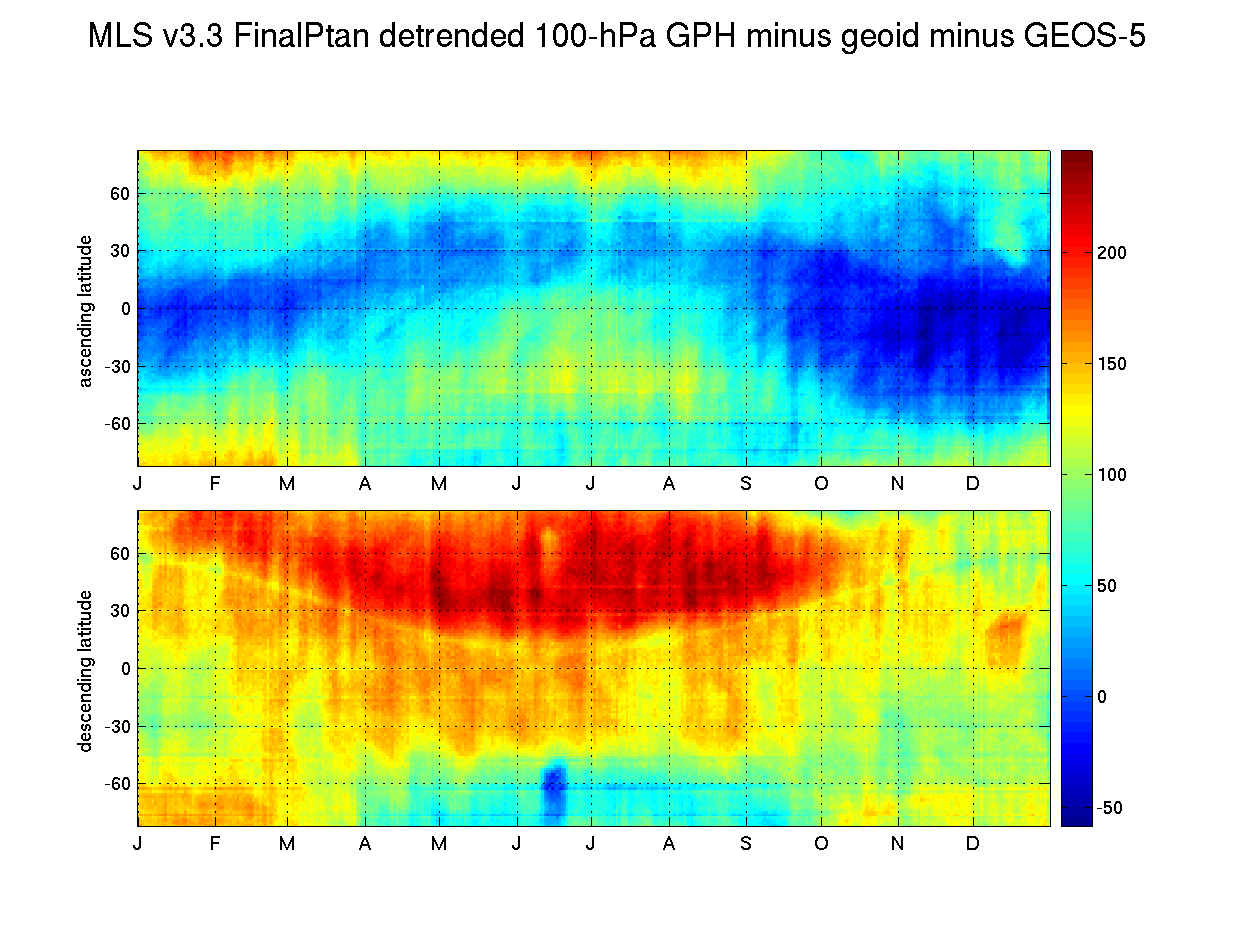
\includegraphics[width=0.7\linewidth]{figures/GPH_geoid_correction2A}
\caption{Annually-repeating biases between MLS 100-hPa GPH and GEOS-5.2
  100-hPa GPH as functions of ascending and descending latitude and of
  day of year.  These biases were computed based upon data from the
  years 2005--2012. (I will remake this figure as a native eps.)}
\label{fig:GPH_lat_annual}
\end{figure}
Some of this annually-repeating ``bias'' is likely annually-repeating
geophysical information captured by MLS that is not in the GEOS-5
analysis, but the large ascending-descending are almost certainly not
primarily diurnal effects.  After removal of this annually-repeating
bias and a there is a residual global decreasing trend in the MLS
100-hPa GPH relative to GEOS-5 of $\sim$100\,m in the first 4 years of
the mission, 2005--2008, with a further $\sim$15\,m decrease in
2009--2012.  The standard deviation of the differences between the
bias-corrected MLS and GEOS-5 100-hpa GPH is on the order of 20\,m.

\subsection*{Differences between \thisv and previous versions}

The \thisv GPH values are typically slightly higher than those of the
v3.3 product, with typical mean differences ranging from 20\,--\,40\,m
in the stratosphere, increasing by $\sim$10\,m in the upper troposphere
and in the mesosphere.  Typical scatter about the mean difference is
$\sim$40\,m at 100\,hPa, increaing to 60\,m at 1\,hPa and 100\,m at
0.01\,hPa.  Seasonal and latitudinal variations in the mean difference
between \thisv and v3.3 GPH are typically less than 20\,m, with somewhat
larger seasonal differences in the high southern latitudes and above
0.01\,hPa.  As with temperature, the 316-hPa level of \thisv GPH is not
recommended for scientific use.  The standard \thisv GPH product is
reported on the same 55-level grid as is the \thisv temperature.

\subsection*{Vertical resolution}

The GPH profile is vertically-integrated temperature, so its vertical
resolution is not well-defined.  The vertical resolution of the
underlying temperature given in Section~\ref{sec:StandardTemperature} is
repeated in Table~\ref{tab:GPHSummary}.

\subsection*{Precision}

MLS \thisv GPH precision is summarized in Table~\ref{tab:GPHSummary}.
Precision is the random component of measurements that will average-down
if a measurement is repeated.  The retrieval software returns an
estimate of GPH precision only for the 100\,hPa reference level, as this
is the only element included in the MLS ``state vector.''  GPH precision
at other standard-product profile levels (summarized in column~2 of
Table~\ref{tab:GPHSummary}) is calculated from the GPH precision at the
reference level and the profile of temperature precisions.  Calculated
precision values are \texttildelow35\,m from 261\,hPa to 100\,hPa,
\texttildelow45\,m at 1\,hPa, \texttildelow110\,m at 0.001\,hPa.
Off-diagonal elements of the temperature/GPH error covariance matrix are
neglected in this GPH-precision-profile calculation, but resulting
errors are believed to be small (\texttildelow5\,m near 100\,hPa.)

\subsection*{Accuracy}

The accuracy of the v2.2 GPH was modeled based upon consideration of a
variety of sources of systematic error, as discussed in
\citep{SchwartzEtal08}. \thisv accuracy is believed to be substantially
similar and the results of the v2.2 calculations are given in column
four of Table\,\ref{tab:GPHSummary}. Of the error sources considered,
modeled amplifier non-linearity had the largest impact, just as is the
case with the calculation for temperature.

The second terms in column four are model-based estimates of the bias
magnitude from other sources including uncertainty in
pointing/field-of-view, uncertainty in spectroscopic parameters, and
retrieval numerics.  The combined bias magnitudes due to these sources
is 100\,--\,150\,m.

``Observed bias uncertainty'' in Table~\ref{tab:GPHSummary} is an
estimate of bias based upon comparisons with analyses and with other
previously-validated satellite-based measurements.  These comparisons
were made using MLS v2.2, but as the biases between v2.2 and \thisv GPH
are generally less than 50\,m from 261\,--0.1\,hPa and reasonably
constant, so these results hold for \thisv as well.  The primary sources
of correlative data were the Goddard Earth Observing System, Version
5.0.1 data assimilation system (GEOS-5) \citep{ReineckerEtal07}, used in
the troposphere and lower stratosphere, and the Sounding of the
Atmosphere using Broadband Radiometry (SABER)
\citep{MlynczakAndRussell95}, used in the upper stratosphere through the
mesosphere.  MLS has a 150\,m high bias relative to analyses (GEOS-5) at
100-hPa that drops to 100\,m at 1\,hPa.  Biases with respect to SABER
are small at 0.1\,hPa but increasingly negative at higher levels,
reaching -600\,m at 0.001\,hPa, but with significant latitudinal and
seasonal variability.

\subsection*{Data screening}

GPH should be screened in the same way as is temperature:

\begin{description}
\item[Pressure range:] \screeningrule{261\,--\,0.001\,hPa.}
  \standardrangestatement

  \standardprecisionrule GPH precision is set negative at and beyond any
  level in the integration of temperature away from the 100-hPa
  reference level where temperature has negative precision.

\evenstatusrule

\item[Clouds:]

  \screeningrule{Thick clouds are believed have some impact on \thisv
    GPH measurements in the upper troposphere (261\,--\,100\,hPa),
    however the cloud-flags bits of the \thisv GPH status are not useful
    in screening out cloud impacts.  Screening of \thisv tropospheric
    GPH for values impacted by clouds is an area of ongoing research.}

\item[Quality:] \qualityrule{0.9} This threshold typically excludes
  1.4\% of global profiles, but 4.8\% of tropical profiles.

\item[Convergence:] \convergencerule{1.021} Use of this threshold
  typically discards 0.1\% of profiles and eliminates a significant
  fraction, but not all of a non-Gaussian tail of outliers that
  comprises less than 0.01\% of the 100-hPa retrieved values.

\end{description}

\subsection*{Review of comparisons with other data sets}
\label{sec:GPHComparisons}

The 100\,hPa reference GPH is typically 100\,--\,250\,m higher than
GEOS-5 in the northern high latitudes and 50\,--\,200\,m higher than
GEOS-5 in the Southern high latitudes. As GPH profiles are calculated
relative to the reference level, biases at 100\,hPa move entire profiles
up and down.  At low latitudes, the GPH observations taken on the
ascending branch of the orbit are typically 0\,--\,120\,m higher than
GEOS-5. while those from descending branch are 100\,--\,200\,m higher.
A seasonal cycle in the daily mean ascending/descending differences of
\texttildelow100\,m peak-to-peak is evident in the high-southern
latitudes (peaking in January) and in the ascending branch of the
equatorial mean differences (peaking in July) There has been a general
downward trend in the MLS minus GEOS-5 bias of 40\,--\,50\,m/year over
the life of the mission.  Like v2.2 GPH, \thisv GPH has a bias of
\texttildelow100\,m at 10\,hPa with respect to GEOS-5 and SABER, and the
bias with respect to SABER becomes increasingly negative at lower
pressures: \texttildelow\,$-$100\,m at 0.01\,hPa and
\texttildelow\,$-$500\,m at 0.001\,hPa.  These negative biases reflect
the general low temperature bias of MLS with respect to SABER.

\subsection*{Desired improvements for future data version(s)}

Reduction of biases in the GPH product likely requires improvement of
our ability to model atmospheric radiative transfer and/or the
measurement system to improve the fit between the forward model and
observed radiances near the O$_2$ spectral lines from which temperature
and pointing information are extracted.  The simple model of ``gain
compression'' proposed during v2.2 validation proved inadequate during
\thisv development, but research in this area is ongoing.  Some
seasonally and latitudinally-repeating systematic errors in GPH may be
the result of error in the absolute pointing reference that is taken
from the spacecraft attitude and ephemeris data stream.  Reduction of
these systematic errors is an area of ongoing research.
  
\begin{table}
\label{tab:GPHSummary}
\begin{minipage}{\linewidth}\small
\centering\begin{tabular}{cccccl}
\toprule
\textbf{Region} & 
\parbox[m]{22mm}{\centering\textbf{Resolution\\ \mbox{Vert. $\times$ Horiz.} / km}} &
\parbox[m]{18mm}{\centering\textbf{Precision\footnote{Precision on individual profiles} \\/ meters}} &
\parbox[m]{20mm}{\centering\textbf{Observed bias\\uncertainty\\ / m}} &
\textbf{Comments} \\
\midrule
$<$0.001\,hPa & --- & --- & --- & --- & Unsuitable for scientific use \\
0.001\,hPa          & 10--13 $\times$ 220  & $\pm$110 & $-$450 & \\
0.01\,hPa           & 8--12 $\times$ 185  & $\pm$85   & $-$100 & \\
0.1\,hPa            & 6 $\times$ 165   & $\pm$60   &  0  & \\
1\,hPa              & 7 $\times$ 165   & $\pm$45   & 100 & \\
10\,hPa             & 4.3 $\times$ 165 & $\pm$35   & 100 & \\
100\,hPa            & 5.2 $\times$ 165 & $\pm$30   & 150 & \\
261\,hPa            & 5.3 $\times$ 170 & $\pm$35   & 150 & \\
1000\,--\,316\,hPa & ---      & ---             & ---     & --- & Unsuitable for scientific use\\
\bottomrule
\end{tabular}
\end{minipage}
\end{table}

%%% Local Variables: 
%%% mode: latex
%%% TeX-master: "v4-x-report"
%%% End: 
